\documentclass[10pt]{article}
\usepackage[letterpaper]{geometry}
\usepackage{listings}
\usepackage{graphicx}
\renewcommand{\figurename}{Imagen}


\title{\textbf{Reporte: Interbloqueos}}
\author{Diego Ruiz Mora | 2202000335}
\date{9-Octubre-2023}

\begin{document}
	
	\maketitle
	\section{Variables Globales}
	Todos los programas contienen un par de variables globales con el mismo propósito en todos los programas.  Notaremos que solo el ultimo de los códigos  usará la variable global que esta comentada, que funcionará para hacer el conteo de veces que se ejecutan los hilos. 
	\begin{figure}[h!]
		\centering
		
\includegraphics[width=\linewidth]{valGob.png}
		\caption{Variables Globales}
		\label{fig:vg}
	\end{figure}
	Encontraremos la variable \emph{almacén} del tipo arreglo de caracteres con una longitud de diez, que servirá para mostrar los productos generados o consumidos. Por otro lado tenemos \emph{condc} y \emph{condp} que son variables de condición que nos permite bloquear los hilos si cumplen ciertas condiciones o igual despertar estos hilos en caso de cumplir ciertas características.  A su vez, tenemos también una variable del tipo mutex \emph{candado}  que nos ayudará a delimitar la región crítica y el acceso de cada uno de los hilos a la misma. Por último las variables enteras de \emph{pos} que indica la posición dentro del almacén y el contador, que ya se mencionó su uso.  
	\section{Funciones del programa}
	Muchas de las funciones de los códigos son iguales, algunas solo varían en una pequeña cosa, de manera conveniente explicaremos la función solamente una vez para ahorrarnos la necesidad de repetirlo en cada uno de los códigos.  
	\subsection{Función Principal}
	Comenzamos por la función principal, donde encontramos la declaración de variables del tipo \textbf{pthread\_t} que serán los dos hilos que utilizamos para consumir y producir elementos dentro del almacén. Para ello tenemos que inicializar las variables de condición para cada uno de los hilos, además hacemos la creación de los hilos dándoles como imagen la función \emph{intentaRegionCritica}, recordemos que tenemos que esperar a que termine de ejecutar cada uno de los hilos creados. 
	\\\\
	Para finalizar destruimos las condiciones y el candado, esto con las ultimas tres instrucciones. donde pasamos por referencia los valores de los respectivos.  
	\begin{figure}[h!]
		\centering
		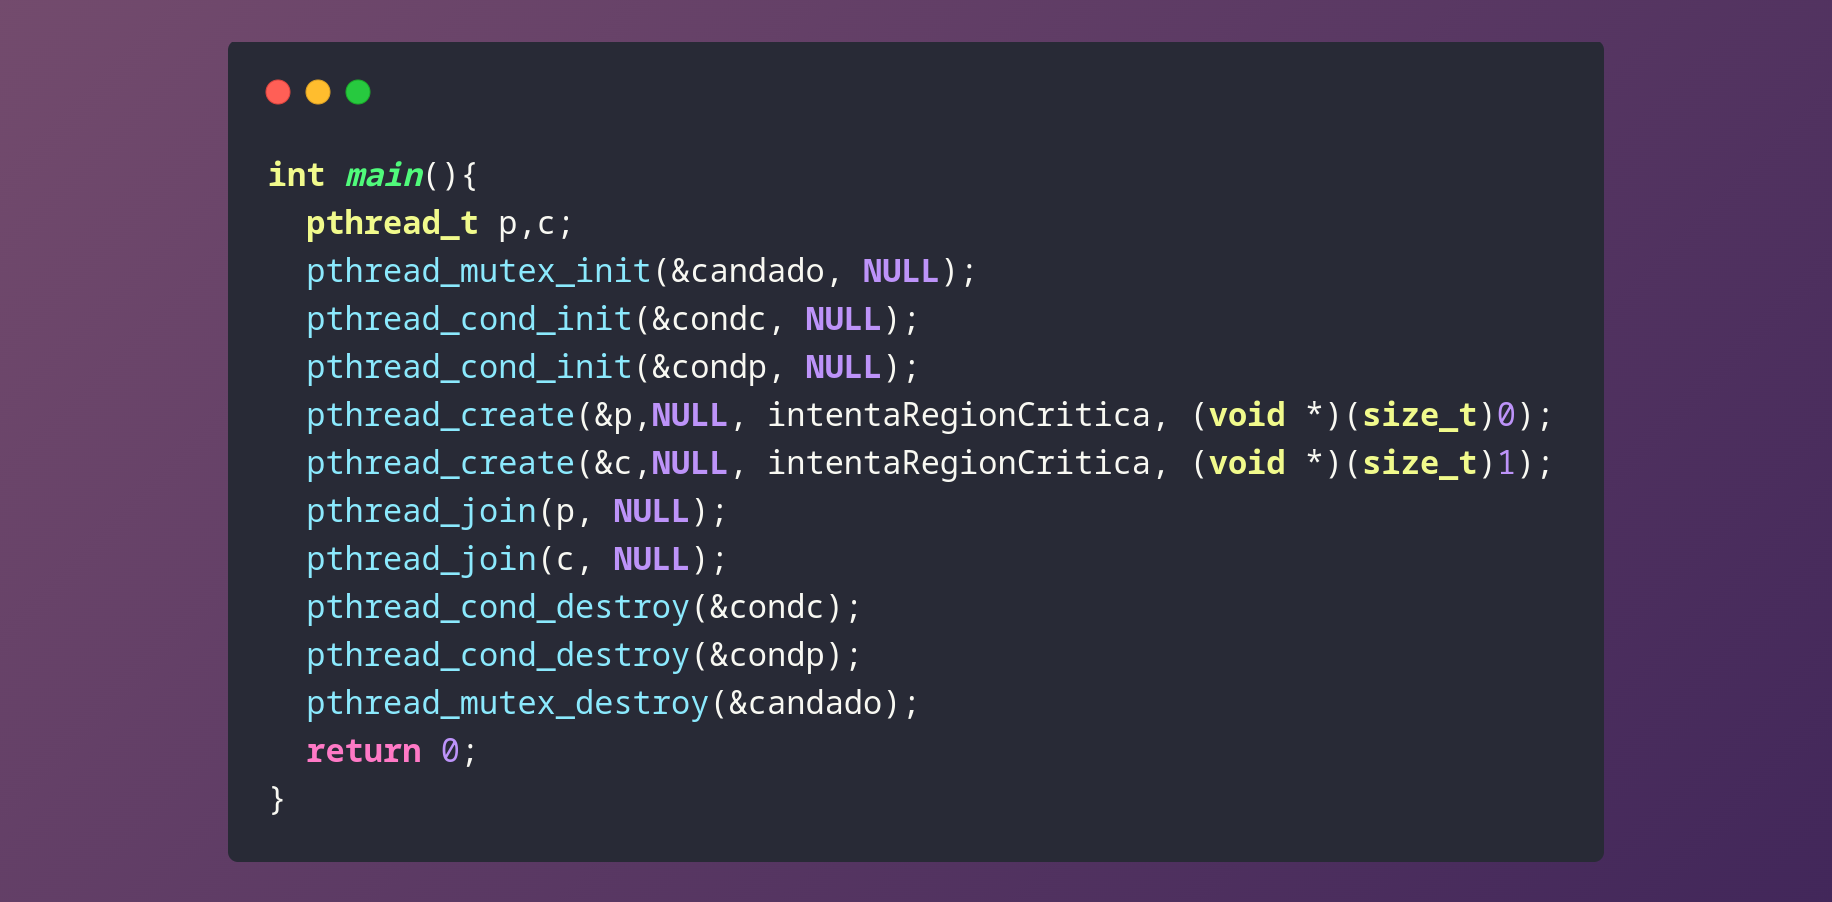
\includegraphics[width=\linewidth]{main.png}
		\caption{Función Principal}
		\label{fig:main}
	\end{figure}
	\subsection{Función para cada hilo}
	La llamada función \emph{intentaRegionCritica} que es la imagen de cada uno de los hilos recibe como parámetro el número de hilo, que justamente nos funcionará para identificar que función particular ejecutará, si la de consumir o la de producir, pero para ello primero tenemos que generar un ciclo de cincuenta repeticiones y dentro de el haremos la delimitación de la región critica para que cada uno de los hilos puedan acceder de manera ordenada  a ella. La delimitación laharemos abriendo y cerrando el mutex, todo esto dentro del ciclo, para que lo repita cincuenta veces por cada uno de los hilos, para darnos un total de cien veces. 
	\begin{figure}[h!]
		\centering
		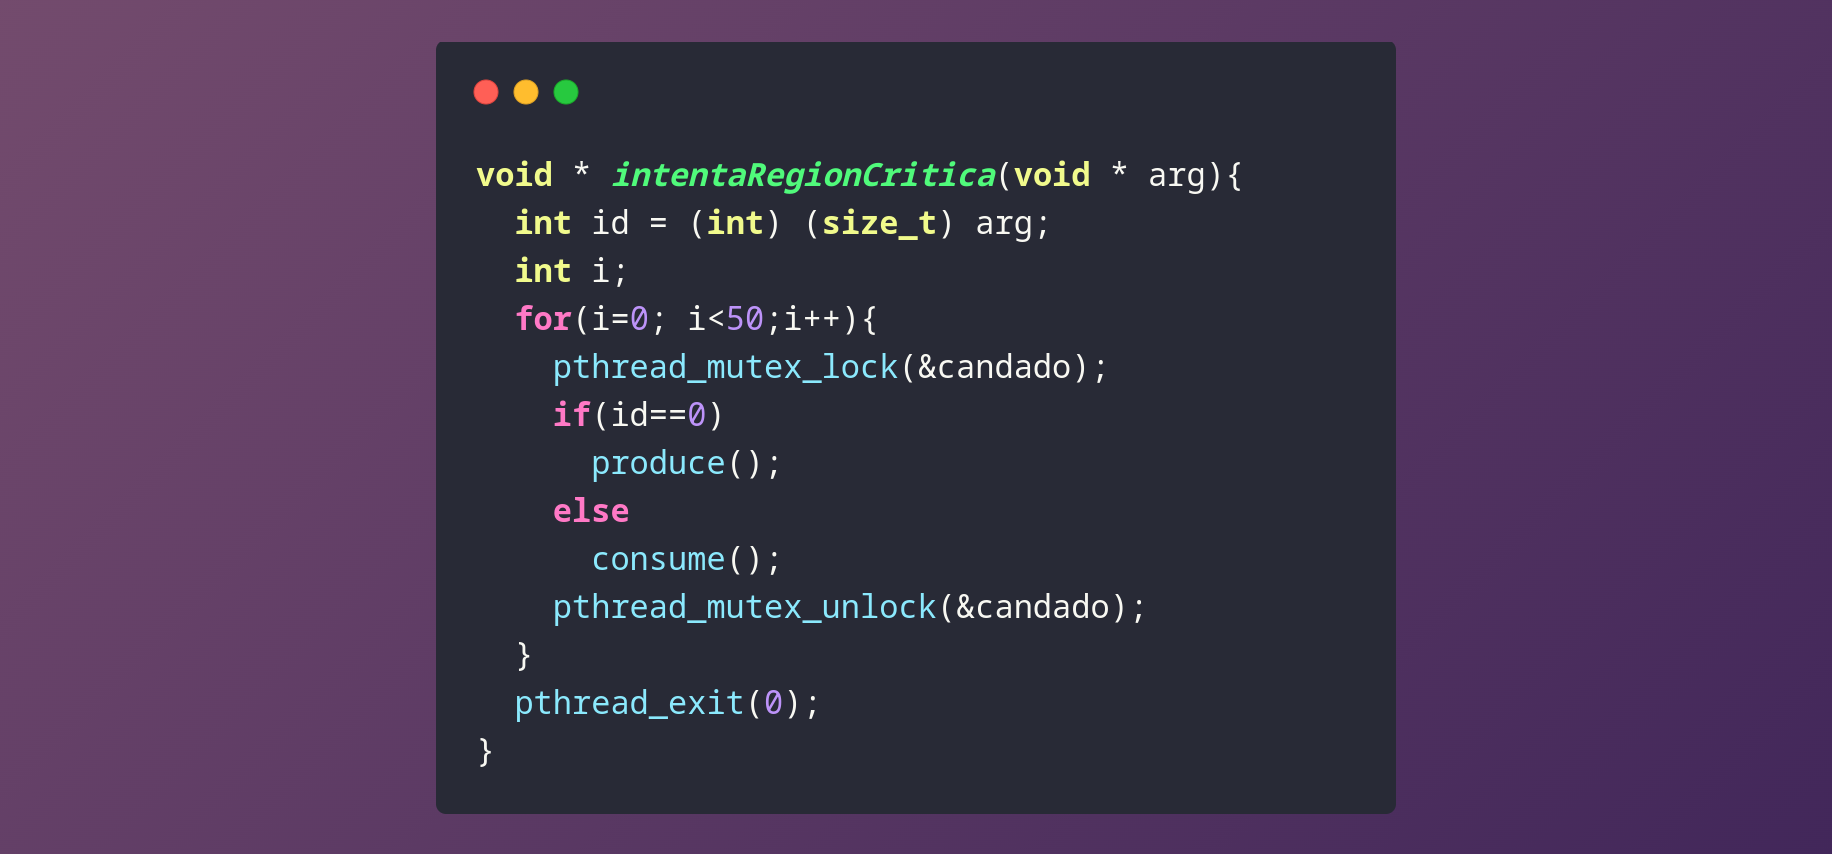
\includegraphics[width=\linewidth]{intentaRC.png}
		\caption{Función intentaRegionCritica}
		\label{fig:intentaRC}
	\end{figure}
	\newpage
	\subsection{Función 'consume'}
	Esta función nos permitirá consumir los productos del almacén para ello utilizamos primero un condicional para el caso donde el la posición del almacén sea igual a cero, esto ocurre porque no tenemos elementos en el almacén, no tiene sentido que consumamos, por lo que se dormirá este proceso. 
	Por otro lado , en cualquier otra posición se debería de consumir  el producto, que en este caso lo hace asignando el carácter nulo y restando uno a posición, para notarlo imprimimos el \emph{almacén} para notar las diferencias. Por ultimo despertamos al otro hilo para que pueda producir. Cabe notar que esta función solamente aplica a los dos primeros códigos, ya que en el tercero necesitaremos otras condicionales, que son muy parecidas. 
	\begin{figure}[h!]
		\centering
		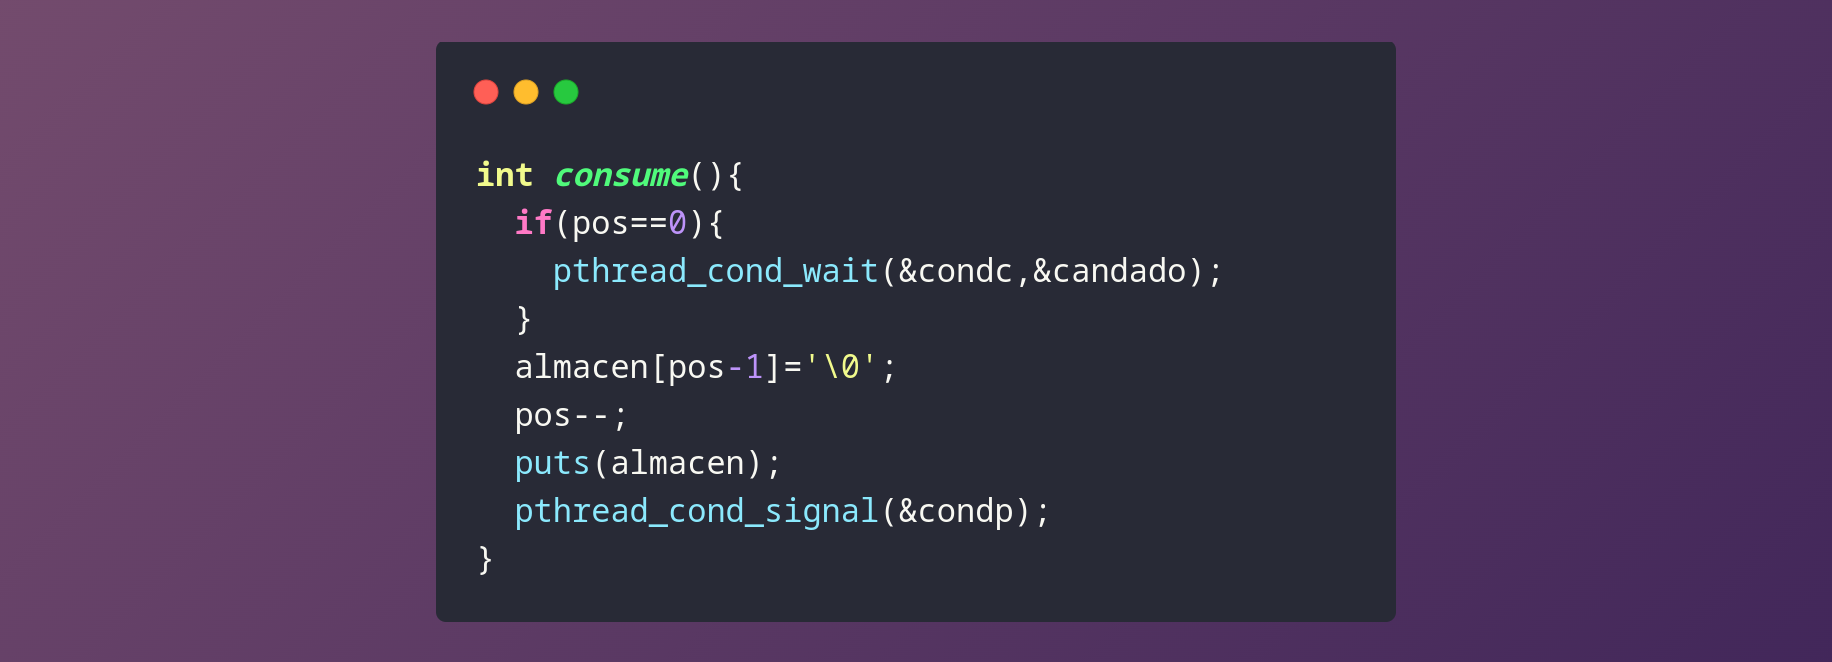
\includegraphics[width=\linewidth]{consume.png}
		\caption{Función 'consume'}
		\label{fig:consume}
	\end{figure}
\end{document}